\section{Metodologia}
\label{sec:metodologia}

Spiegare notazione grafo, parametri, usiamo 1 simbolo per indicare gli score. Quando scriviamo una sezione qui sotto 2.x, se ci serve della notazione poi andiamo a metterla qui. 
Fare dei paragrafi per BM25, PageRank, Hits, LSA, ES.

%In questo paragrafo, si illustreranno i metodi sviluppati e sperimentati con le
%attivit\`a di laboratorio. Le notazioni e tutti gli aspetti non banali dovranno
%essere spiegati. Naturalmente, la notazione di un paragrafo non dovr\`a essere
%reintrodotta nei paragrafi successivi, di conseguenza, la notazione non dovr\`a
%essere ambigua.

\subsection{Approccio}
\label{sec:approccio}

%Vogliamo max la map. Usando treceval spiegare cos'e'. Spiegare brevemente il lavoro, molto veloce dire che abbiamo lavorato insieme dopo la prima sessione in lab. Usato python, con \texttt{numpy} per matrici, matplotlib per plottare, networkx per grafi, git per versionamento, latex per i report.
%Il nostro scopo e' ottenere un valore di map il piu' elevato possibile. Per calcolarla e verificarne il cambiamento durante le varie versione del codice utilizziamo \texttt{treceval}, esso e' il tool standard usato dalla "TREC community" per valutare un'esecuzione ad hoc, dandole il file contenete i risultati e un set standard di risultati giudicati.  

%Abbiamo deciso di utilizzare un approccio probabilistico poiche' fornisce una formalizzazione piu' pulita di cosa volgiamo che faccia un sistema IR: dare documenti rilevanti agli utenti. 
%Inoltre per via delle nostre conoscenze abbiamo voluto utilizzare il linguaggio Python per dare corpo ai progetti. Inoltre vi sono diverse librerie che implementano molti metodi utili per tale corso e per garantire buone performance al codice: \texttt{numpy} usata per la gestione delle matrici, \texttt{matplotlib} utilizza per effettuare i plot (grafici) dei risultati ottenuti, \texttt{networkx} utilizzata per la creazione e gestione dei grafi.
%Oltre a \texttt{Python} abbiamo utilizzato altri software per il lavoro. E' stato usato \texttt{Git}, e' un sistema di versionamento distribuito, per lo scambio del codice e l'aggiornamente delle diverse versioni di quest'ultimo. Infini \texttt{latex} per la scrittura dei pdf di report.
%Per ogni esercitazioni è stato utilizzato un approccio di gruppo. Dopo la prima sessione di laboratorio di ogni esercitazione ci siamo ritrovati per la scrittura del codice, la discussione sui risultati e la stesione del report.

\subsection{Indicizzazione} \label{sec:metodi-di-indic}

Qui va il contenuto del laboratorio n. 2.

\subsection{Reperimento}
\label{sec:metodi-di-reper}

Qui va il contenuto del laboratorio n. 3. Esso rappresenta la \textit{baseline}.

\subsection{Relevance Feedback}
\label{sec:relevance-feedback}

Qui va il contenuto del laboratorio n. 4.

\subsection{PageRank}
\label{sec:pagerank}

Qui va il contenuto del laboratorio n. 5.

\subsection{Latent Semantic Analysis}
\label{sec:lsa}

Qui va il contenuto del laboratorio n. 6.

\subsection{Hyper-linked Induced Topic Search}
\label{sec:hits}

Qui va il contenuto del laboratorio n. 7.

\subsection{Evolution Strategy}
\label{sec:es}

Per ottimizzare gli algoritmi di reperimento abbiamo scelto di utilizzare un Evolution Strategy~\cite{back1996evolutionary} (ES) che e' una tecnica di ottimizzazione basata sui principi che regolano l'evoluzione. Tecniche di questo tipo sono piu' robuste rispetto ai metodi di ricerca lineare per quanto riguardo i massimi locali. Il loro svantaggio consiste nel maggior numero di valutazioni richieste. Nel nostro contesto una valutazione impiega circa 3-10 secondi a seconda della complessita' del metodo di reperimento. Cio' permette di eseguire l'algoritmo di ottimizzazione in un tempo accettabile.

I parametri che abbiamo scelto di ottimizzare cambiano in base alla tecnica di reperimento (e quindi del laboratorio). Per il laboratorio 3 abbiamo scelto di ottimizzare $k_1, b$, ignoriamo $k_2$ in quando abbiamo visto che non ci sono termini ripetuti nelle query e quindi tale termine non influisce sul punteggio. Per il laboratorio 5 ottimizziamo $k_1, b, \alpha$. Per il laboratorio 7 ottimizziamo $k_1, b, \alpha, \beta, \gamma$. La funzione da massimizzare e' la Mean Average Precision.

Figura \ref{fig:es_all} riporta l'andamento della MAP durante l'ottimizzazione della funzione di reperimento dei laboratori. 
\begin{figure*}
        \centering
        \begin{subfigure}[b]{0.475\textwidth}
            \centering
            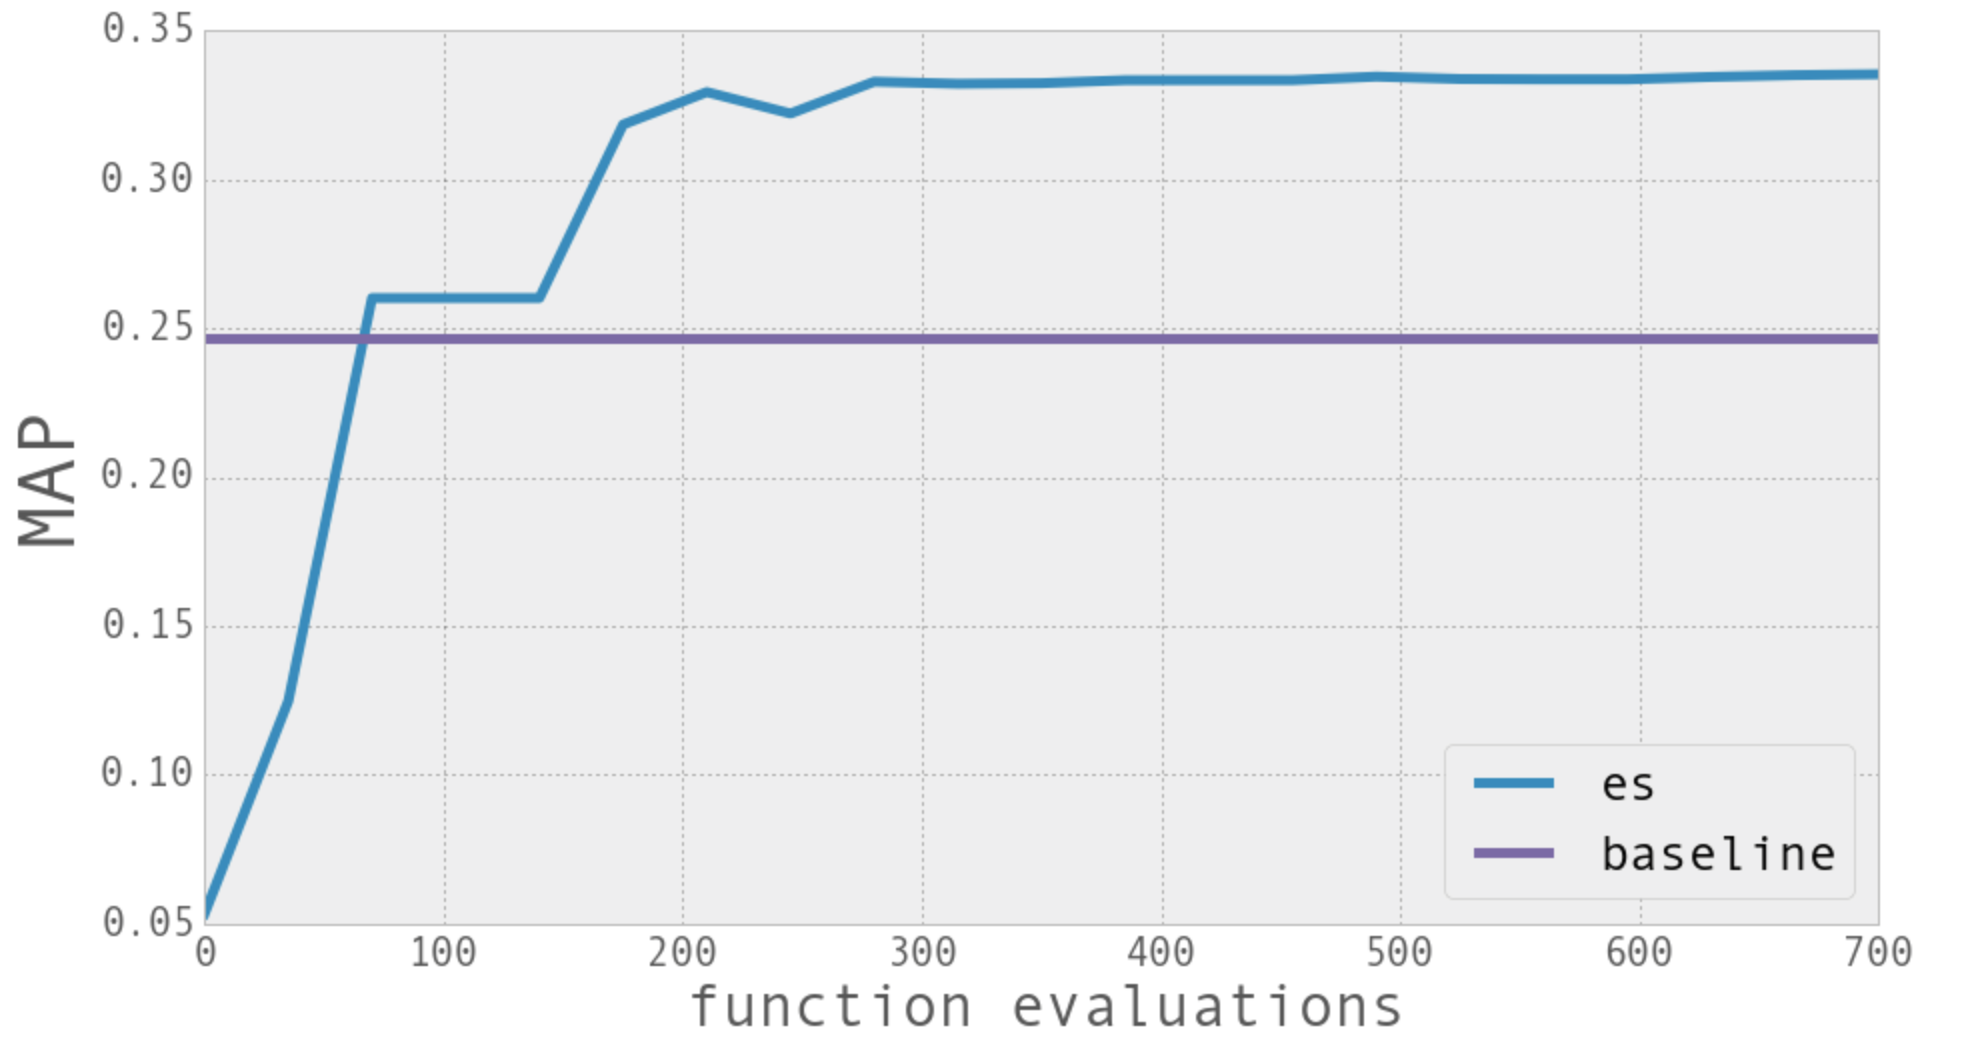
\includegraphics[width=\textwidth]{figures/es_lab3.png}
            \caption[Network2]%
            {{\small Laboratorio 3 (baseline)}}    
            \label{fig:es_lab3}
        \end{subfigure}
        \hfill
        \begin{subfigure}[b]{0.475\textwidth}  
            \centering 
            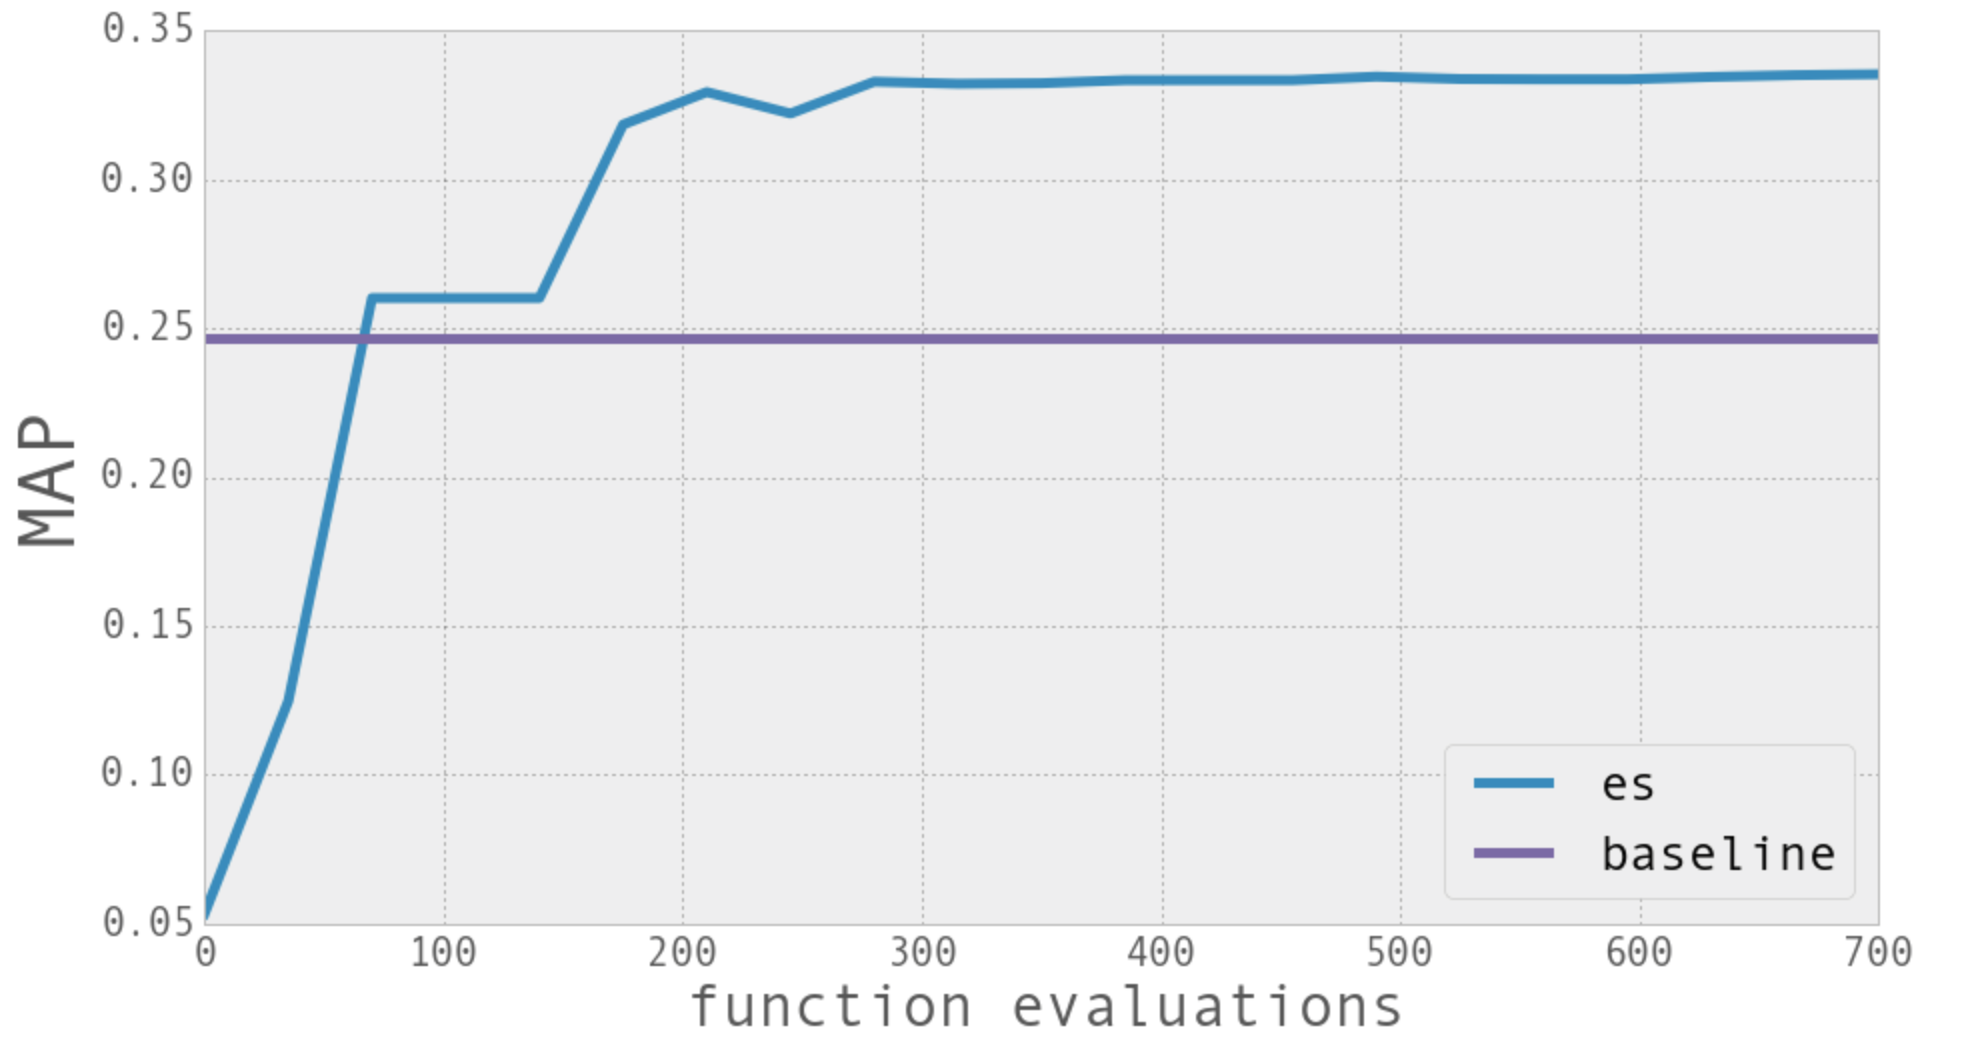
\includegraphics[width=\textwidth]{figures/es_lab3.png}
            \caption[]%
            {{\small Laboratorio 4 (relevance feedback esplicito)}}    
            \label{fig:es_lab4_esp}
        \end{subfigure}
        \vskip\baselineskip
        \begin{subfigure}[b]{0.475\textwidth}   
            \centering 
            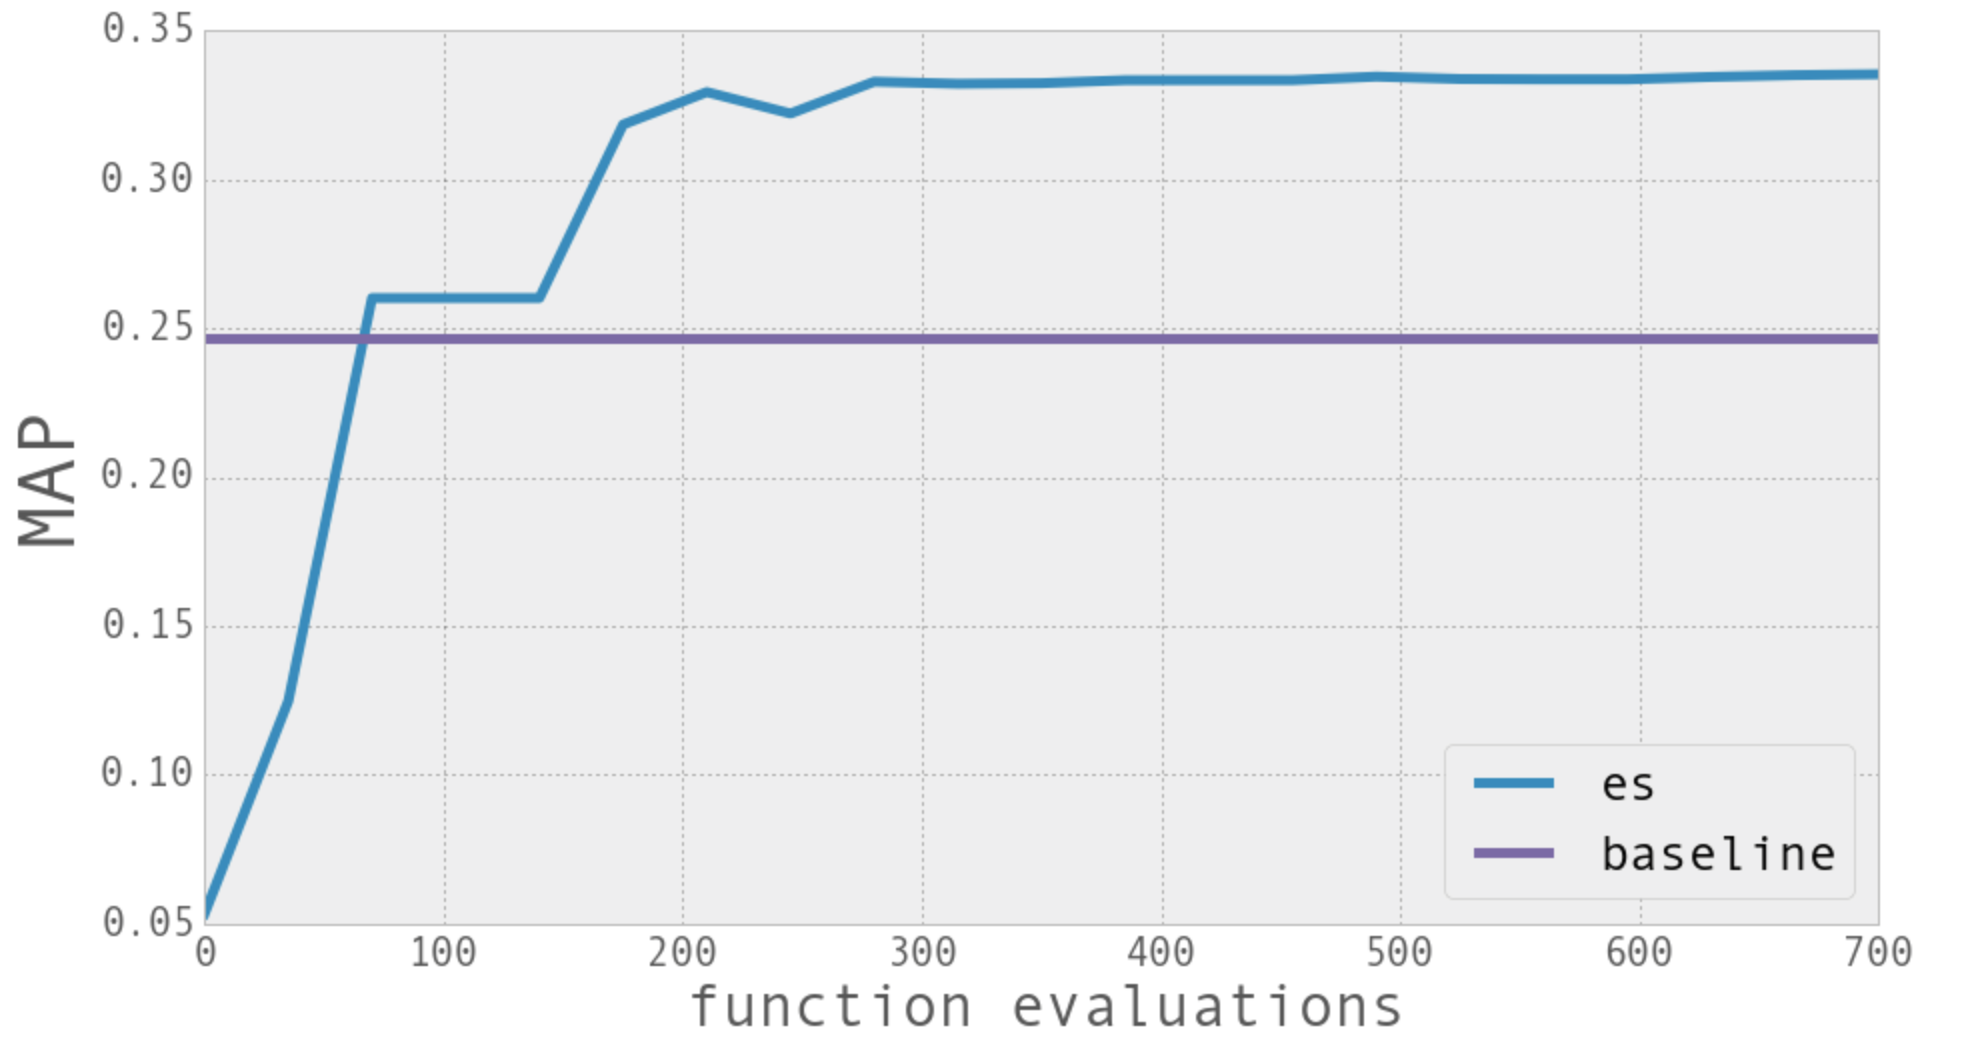
\includegraphics[width=\textwidth]{figures/es_lab3.png}
            \caption[]%
            {{\small Laboratorio 4 (relevance feedback pseudo)}}    
            \label{fig:es_lab4_pse}
        \end{subfigure}
        \quad
        \begin{subfigure}[b]{0.475\textwidth}   
            \centering 
            \includegraphics[width=\textwidth]{figures/es_lab5.png}
            \caption[]%
            {{\small Laboratorio 5 (\textsc{pagerank})}}    
            \label{fig:es_lab5_esp}
        \end{subfigure}
        \vskip\baselineskip
        \begin{subfigure}[b]{0.475\textwidth}  
            \centering 
            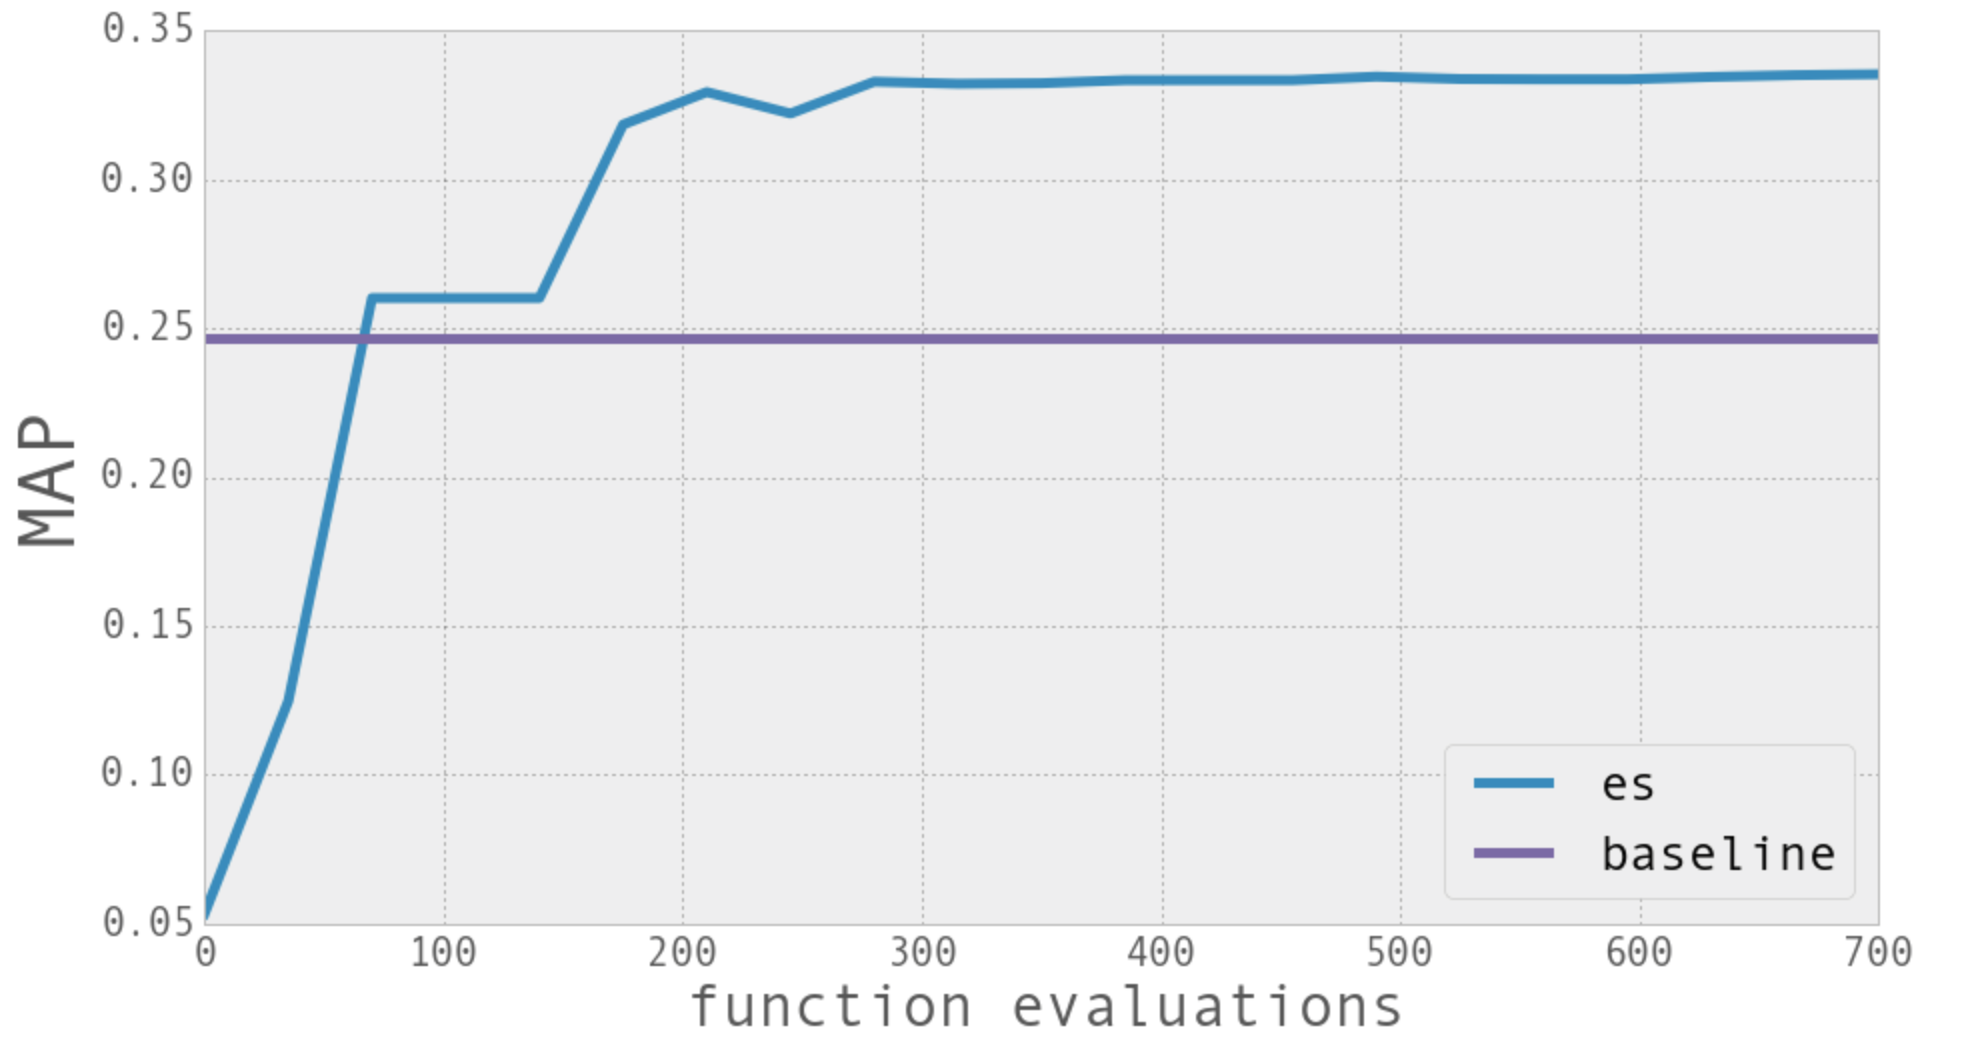
\includegraphics[width=\textwidth]{figures/es_lab3.png}
            \caption[]%
            {{\small Laboratorio 6 (\textsc{lsa})}}    
            \label{fig:es_lab6}
        \end{subfigure}
        \quad
        \begin{subfigure}[b]{0.475\textwidth}   
            \centering 
            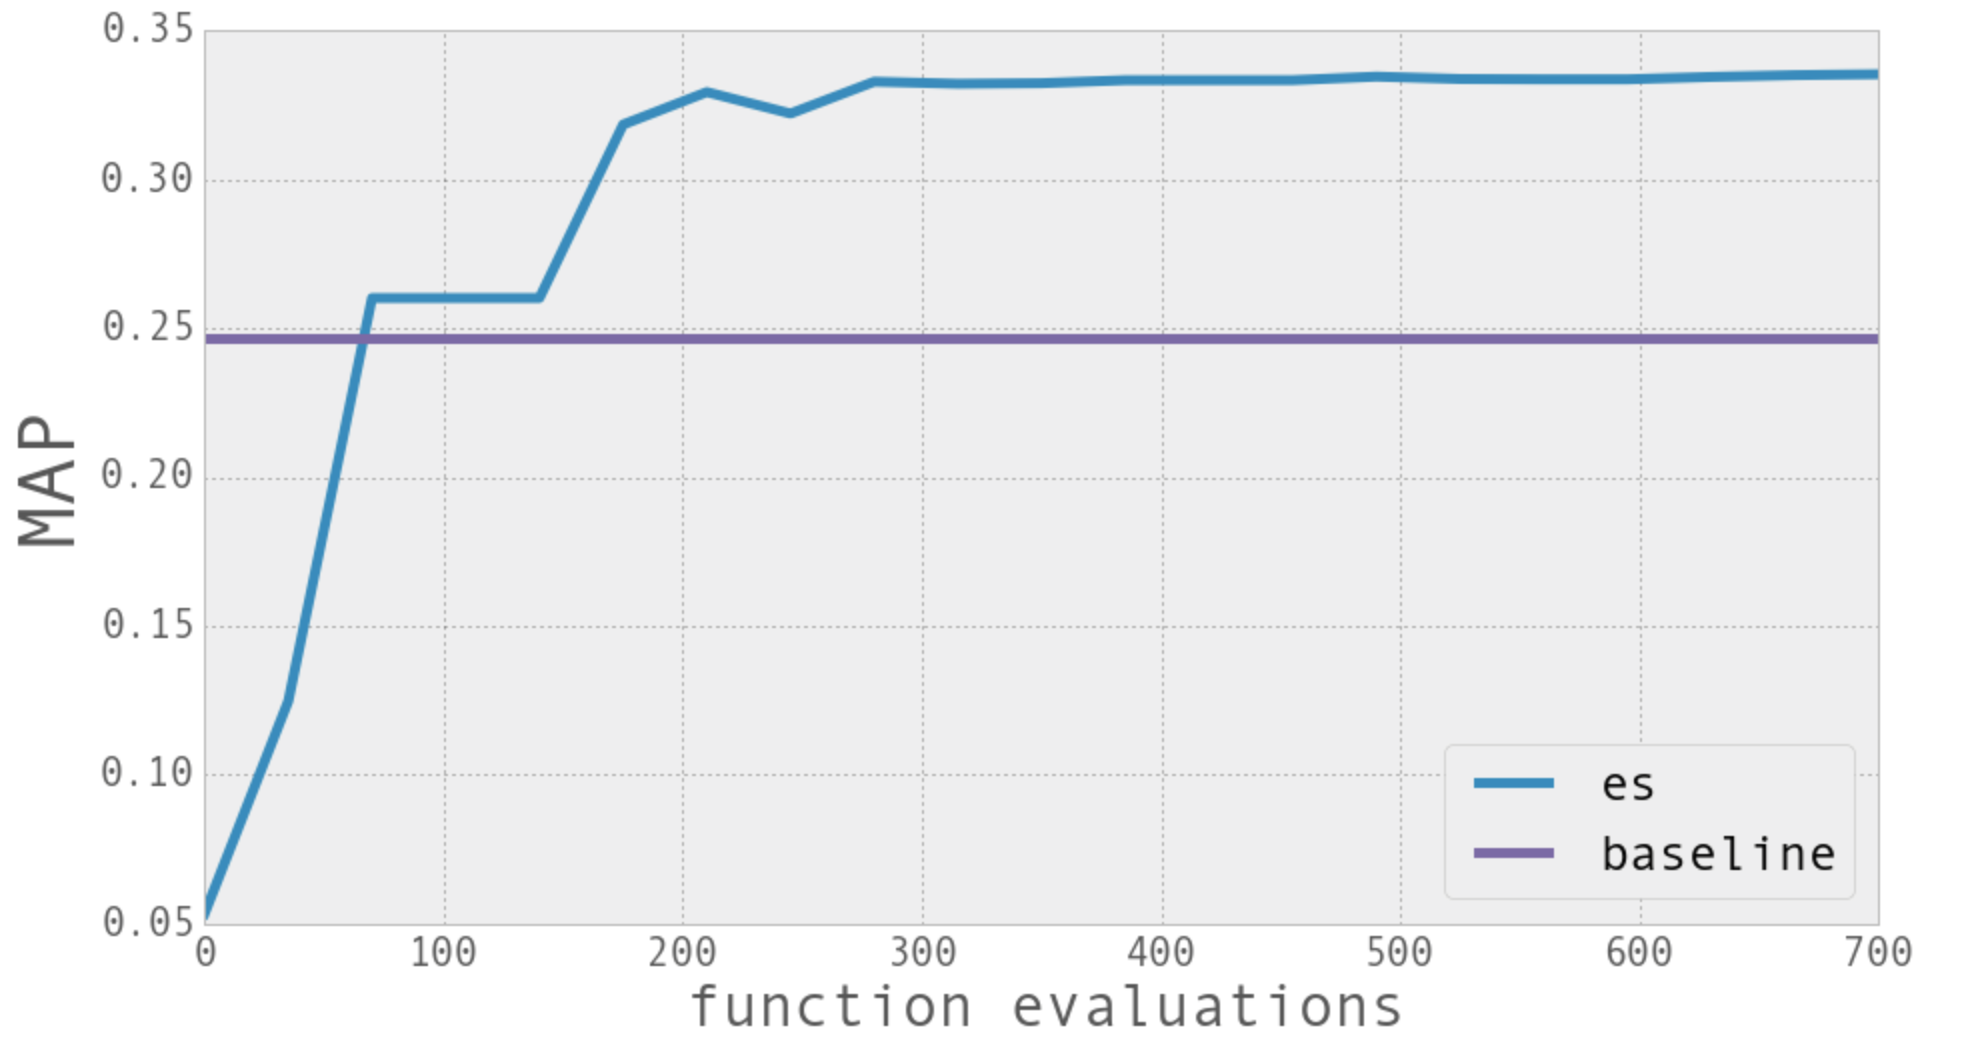
\includegraphics[width=\textwidth]{figures/es_lab3.png}
            \caption[]%
            {{\small Laboratorio 7 (\textsc{hits})}}    
            \label{fig:es_lab7}
        \end{subfigure}
        \caption[ The average and standard deviation of critical parameters ]
        {\small The average and standard deviation of critical parameters: Region R4} 
        \label{fig:es_all}
\end{figure*}


%\begin{figure}
%	\centering
%	\begin{subfigure}{.5\textwidth}
%		\centering
%		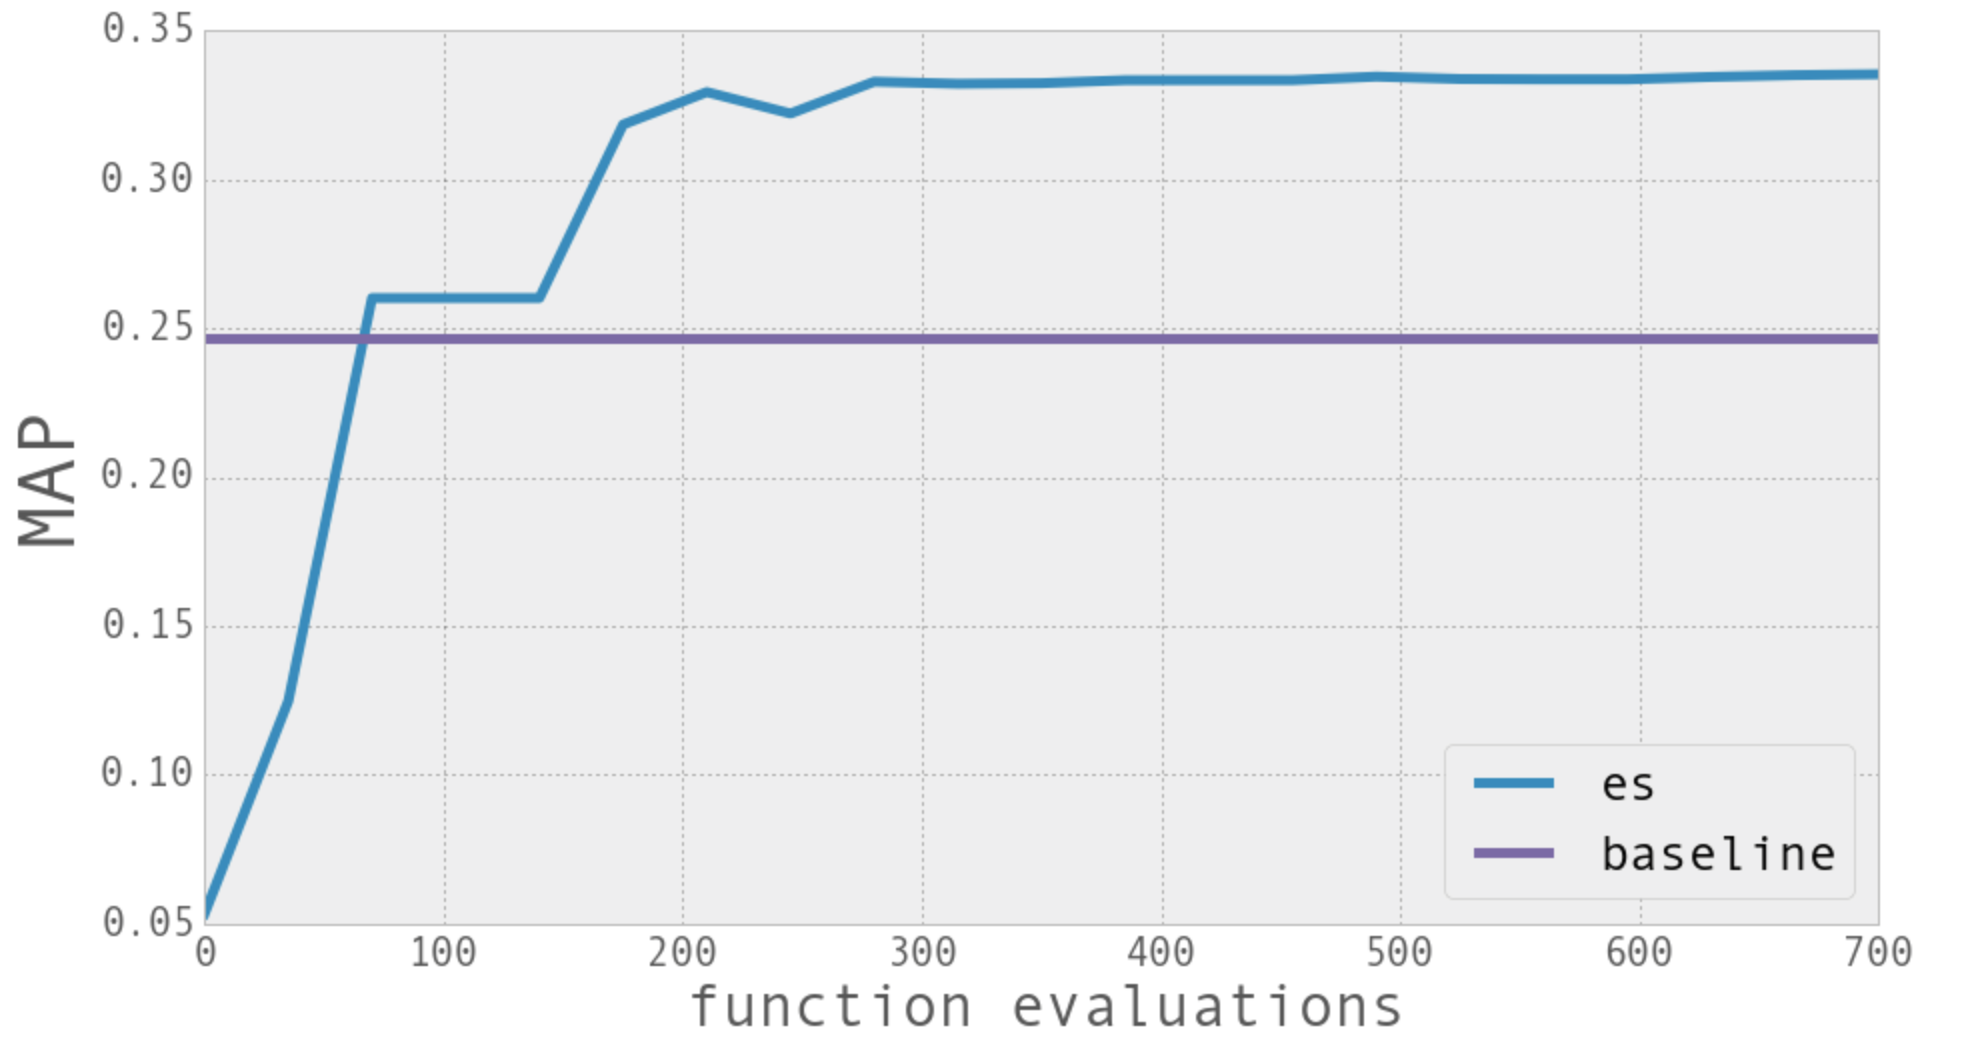
\includegraphics[width=1\textwidth]{figures/es_lab3.png}
%		\caption{MAP durante iterazioni dell'ES per il laboratorio 3.}
%		\label{fig:uno}
%	\end{subfigure}%
%	\begin{subfigure}{.5\textwidth}
%		\centering
%		\includegraphics[width=1\textwidth]{figiures/es_lab5.png}
%		\caption{Grafo base ($B_{56}$).}
%		\label{fig:due}
%	\end{subfigure}
%	\caption{MAP durante iterazioni dell'es}
%	\label{fig:unodue}
%\end{figure}

\begin{figure}[htbp]
	\begin{center}
		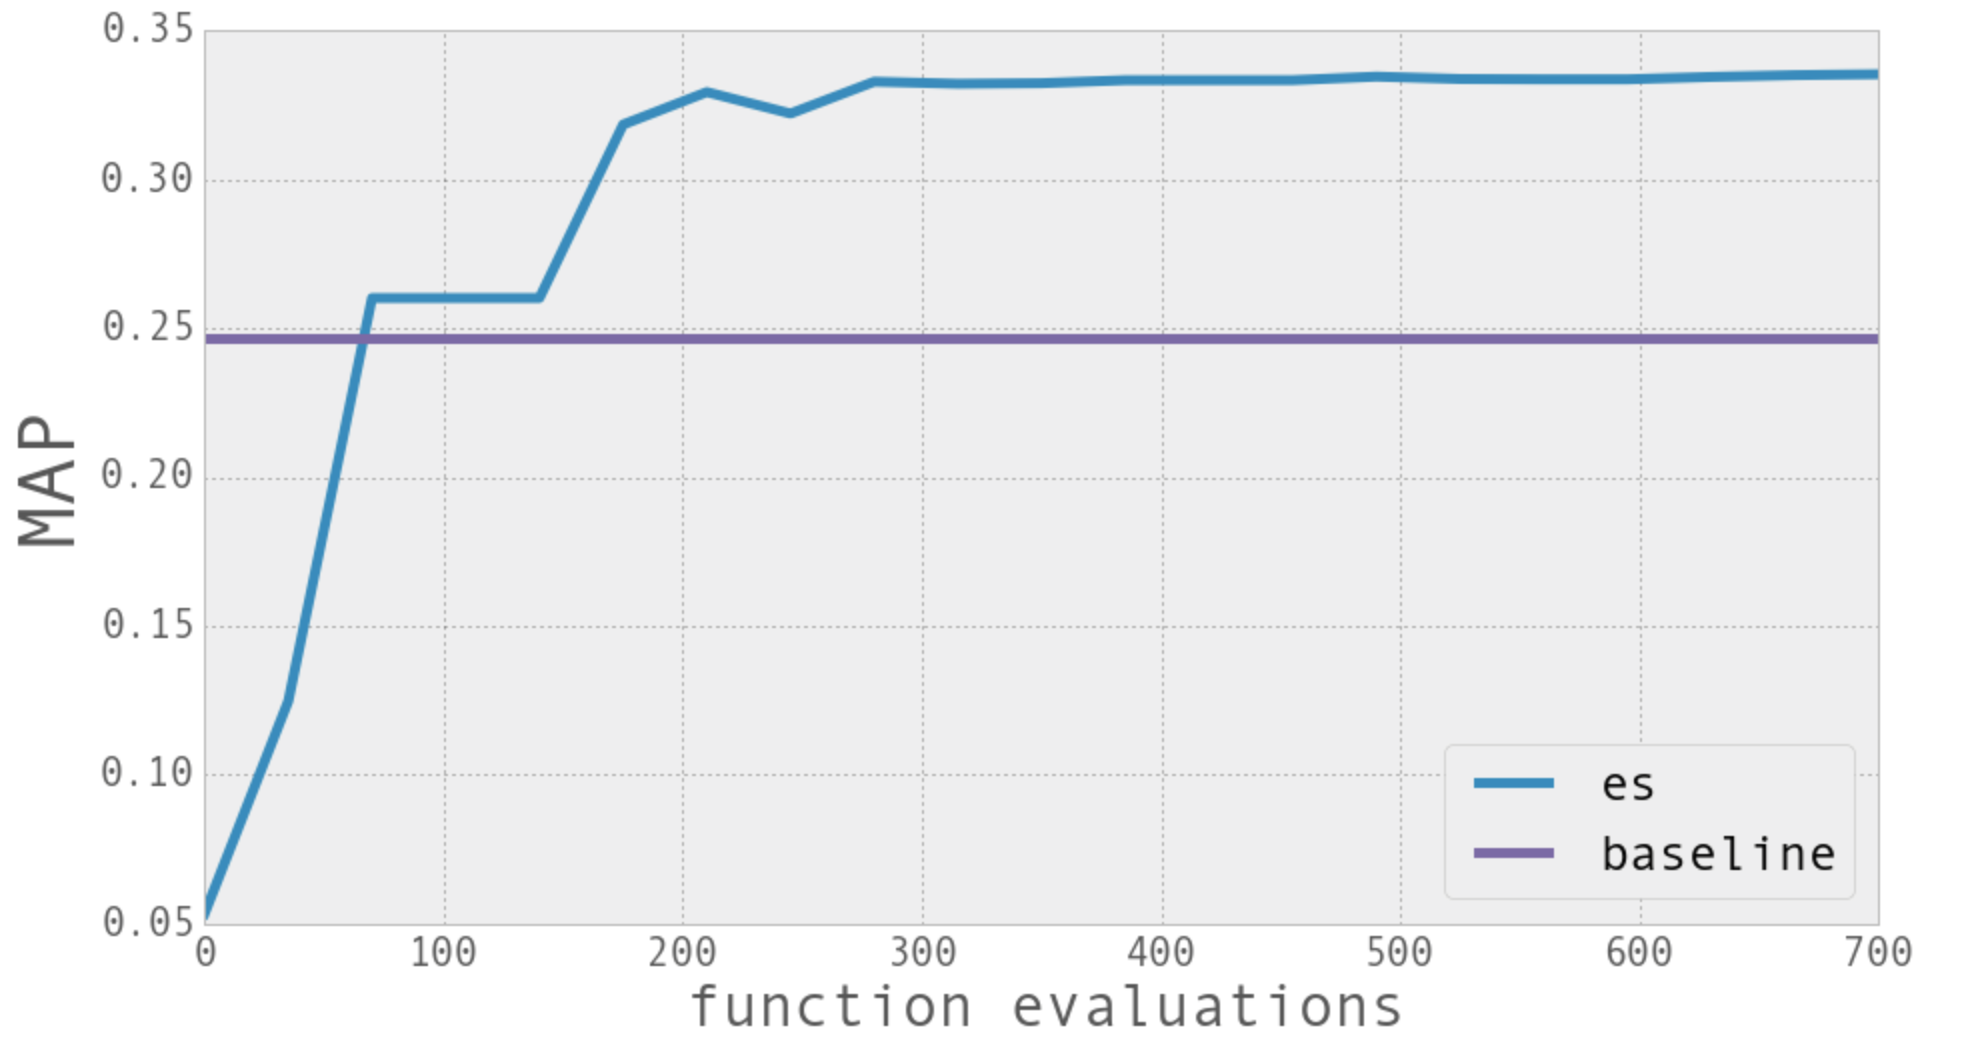
\includegraphics[width=0.75\textwidth]{figures/es_lab3.png}
		\caption{MAP durante ottimizzazione laboratorio 3.}
		\label{fig:es_lab3}
	\end{center}
\end{figure}
\begin{figure}[htbp]
	\begin{center}
		\includegraphics[width=0.75\textwidth]{figures/es_lab5.png}
		\caption{MAP durante ottimizzazione laboratorio 5.}
		\label{fig:es_lab5}
	\end{center}
\end{figure}
\begin{figure}[htbp]
	\begin{center}
		\includegraphics[width=0.75\textwidth]{figures/es_lab5.png}
		\caption{MAP durante ottimizzazione laboratorio 7.}
		\label{fig:es_lab7}
	\end{center}
\end{figure}

Tabella \ref{tab:es} riporta i risultati dell'ottimizzazione.
\begin{table}[htdp]
\caption{Risultati ottimizzazione con ES per i vari laboratori.}
\begin{center}
\begin{tabular}{|c|c|c|}
\hline
laboratorio & parametri & MAP \\
 \hline
3 & $k_1 = 0.0253, b = 0.0221$ & $0.3354$ \\
5 & $k_1 = 0.0237, b = 0.0, \alpha=0.7832$ & $0.3366$ \\
7 & $k_1 = 0.0237, b = 0.0, \alpha=0.7832$ & $0.3366$ \\
\hline
\end{tabular}
\end{center}
\label{tab:es}
\end{table}

Come si puo' vedere grazie all'ES si e' ottenuto un notevole miglioramento in termini di MAP rispetto alla nostra prima versione. I risultati dell'ottimizzazione vengono discussi in Sezione \ref{sec:risult-sper}.

\subsection{Altri metodi}
tipo lucene
\label{sec:altri-metodi}

Se sono stati sviluppati altri metodi, descriverli qui.

